% Condition E (Seed + Taxonomy) - Mechanism Hierarchy
\begin{figure}[H]
\centering
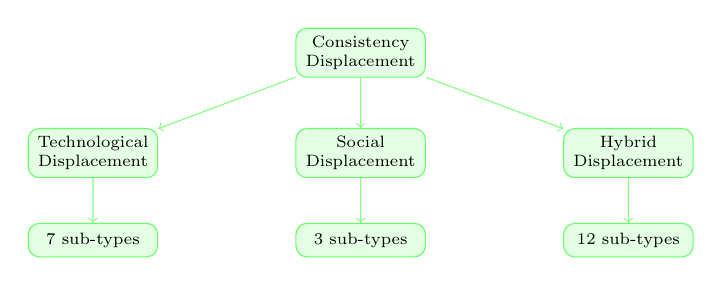
\begin{tikzpicture}[scale=0.85, transform shape,
  grow=south,
  level 1/.style={sibling distance=4cm, level distance=1.5cm},
  level 2/.style={sibling distance=2cm, level distance=1.3cm},
  every node/.style={rectangle, rounded corners, draw=green!60, fill=green!10, font=\scriptsize, align=center, text width=1.7cm, minimum height=0.5cm},
  edge from parent/.style={draw, green!50, ->},
]
\node {Consistency\\Displacement}
  child {node {Technological\\Displacement}
    child {node {7 sub-types}}}
  child {node {Social\\Displacement}
    child {node {3 sub-types}}}
  child {node {Hybrid\\Displacement}
    child {node {12 sub-types}}}
;
\end{tikzpicture}
\caption{Condition E mechanism-tree schematic. The dominant curated backbone divides Consistency Displacement into technological, social, and hybrid branches; compressed boxes summarize lower mechanism categories, while solution nodes and candidate-to-mechanism links are omitted. Four additional candidate-text mechanism roots retained in the database are not shown, yielding the five-root total in Table~\ref{tab:graph-stats}.}
\label{fig:tree-e}
\end{figure}
